\documentclass{beamer}
\usepackage{graphicx}
\usepackage{tikz}
\usepackage{amsmath, amssymb}

\usepackage{tkz-graph}
\usepackage{xcolor}
% Theme
\usetheme{Madrid} % You can change this to other themes like Berlin, CambridgeUS, etc
% Customizing colors
\definecolor{myred}{RGB}{180, 0, 0}
\definecolor{darkred}{RGB}{120, 0, 0}
\setbeamercolor{structure}{fg=myred}
\setbeamercolor{frametitle}{fg=white, bg=myred}
\setbeamercolor{title}{fg=white, bg=myred}
\setbeamercolor{block title}{fg=white, bg=darkred}
\setbeamercolor{block body}{fg=black, bg=white}



% Title Page
\title{Analysis of Algorithm}
\subtitle{Extended Karatsuba, Graph}
\author{Instructor: Dr. Mudassir Shabbir}
\institute{ITU}
\date{February 23, 2025}


\AtBeginDocument{
    \setbeamertemplate{logo}{%
        \hspace*{0.8\textwidth} % Adjust position
        \includegraphics[width=1cm]{Itu.jpg} % Adjust size as needed
    }
}

\begin{document}
\begin{frame}
    \titlepage
    \vspace{1cm}
    \textbf{Scribe:}
 Abdul Basit \\ \ \ \ \ \ \ \ \ \ \ \ Muhammad Okasha Khan
\end{frame}




% Slide 4:Recap Counting Sort
\begin{frame}{Recap Counting Sort}
    \textbf{Concept:} 
    \begin{itemize}
        \item Counts occurrences of each unique element.
        \item Uses this count to determine final positions in sorted order.
    \end{itemize}
    \textbf{Time Complexity:}
    \begin{itemize}
        \item Best/Average/Worst: $O(n + k)$ (where $k$ is the range of numbers)
    \end{itemize}
    \textbf{Stable:} Yes. \newline
    \textbf{Limitation:} Inefficient for large ranges.
\end{frame}

% Slide 5:Recap Bucket Sort
\begin{frame}{Recap Bucket Sort}
    \textbf{Concept:} 
    \begin{itemize}
        \item Distributes elements into multiple "buckets".
        \item Each bucket is sorted individually using another sorting algorithm.
    \end{itemize}
    \textbf{Time Complexity:}
    \begin{itemize}
        \item Best/Average: $O(n + k)$ (where $k$ is the number of buckets)
        \item Worst: $O(n^2)$ (if all elements land in one bucket)
    \end{itemize}
    \textbf{Stable:} Yes (if the inner sorting algorithm is stable).
\end{frame}



% Slide 6:Recap Radix Sort
\begin{frame}{Recap Radix Sort}
    \textbf{Concept:} 
    \begin{itemize}
        \item Sorts numbers digit by digit, starting from the least or most significant digit.
        \item Uses a stable sorting algorithm (like Counting Sort) at each step.
    \end{itemize}
    \textbf{Time Complexity:}
    \begin{itemize}
        \item Best/Average/Worst: $O(d(n + k))$ (where $d$ is the number of digits, $k$ is the base)
    \end{itemize}
    \textbf{Stable:} Yes. \newline
    \textbf{Limitation:} Requires extra space and works best when the number of digits is not too large.
\end{frame}

% Slide 7: Extension of Karatsuba (Toom-3)
\begin{frame}{Extended Karatsuba}
    \textbf{As discussed in Lecture \#7, Karatsuba is an algorithm that multiplies two integers by dividing them into two parts, achieving a time complexity of \(O(n^{\log_2 3}) \approx O(n^{1.585})\).}
    
    \begin{itemize}
        \item Let two numbers:
        \[
        P = [\_\_\_\_A\_\_\_\_\mid\_\_\_\_B\_\_\_\_]  
        \]
        \[
        Q = [\_\_\_\_X\_\_\_\_\mid\_\_\_\_Y\_\_\_\_]  
        \]
        We make three recursive calls, Hence:
        \item \textbf{Recurrence Relation:}
        \[
        T(n) = 3T(n/2) + O(n)
        \]
        \item \textbf{Master Theorem:}  
        \[
        T(n) = \Theta(n^{\log_2 3})
        \]
    \end{itemize}
\end{frame}


% Slide 8: TOOM-3 Algorithm
\begin{frame}{TOOM-3 Algorithm}
    \textbf{Concept:} 
    \begin{itemize}
        \item TOOM-3 is an extension of Karatsuba's multiplication algorithm.
        \item It divides an integer into 3 parts and performs multiplication on them.
        \item The goal is to reduce recursive calls and minimize operations.
    \end{itemize}
    \textbf{Integer Representation:}
    \begin{align*}
        P &= [\_\_\_\_a\_\_\_\_|\_\_\_\_b\_\_\_\_|\_\_\_\_c\_\_\_\_] \quad \text{(n bits)}
    \end{align*}
    \begin{align*}
        Q &= [\_\_\_\_x\_\_\_\_|\_\_\_\_y\_\_\_\_|\_\_\_\_z\_\_\_\_] \quad \text{(n bits)}
    \end{align*}
    \textbf{Assumption:} 
    \begin{itemize}
        \item $n$ is divisible by 3 to allow equal partitioning.
    \end{itemize}
\end{frame}

% Slide 11: TOOM-3 Multiplication Expansion
\begin{frame}{TOOM-3 Multiplication Expansion}
    \textbf{Multiplication:}
    \begin{align*}
        P \times Q &= (a \cdot 2^{\frac{2n}{3}} + b \cdot 2^{\frac{n}{3}} + c) \times (x \cdot 2^{\frac{2n}{3}} + y \cdot 2^{\frac{n}{3}} + z) \\
                   &= (\textcolor{green}{ax\cdot 2^{\frac{4n}{3}}} + \textcolor{red}{ay \cdot 2^n} + \textcolor{blue}{az \cdot 2^{\frac{2n}{3}}} + \\
                   & \quad \ \ \ \ \ \ \ \ \ \ \ \ \ \ \ \textcolor{red}{bx \cdot 2^n} + \textcolor{blue}{cx \cdot 2^{\frac{2n}{3}}} + \\
                   & \ \ \ \quad \textcolor{green}{cz} + \ \ \ \ \ \textcolor{purple}{bz \cdot 2^{\frac{n}{3}}} + \textcolor{blue}{by \cdot 2^{\frac{2n}{3}}} + \\
                   & \quad \ \ \ \ \ \ \ \ \ \ \ \ \ \ \textcolor{purple}{cy \cdot 2^{\frac{n}{3}}})
    \end{align*}
    
    \textbf{Separation:}
    \begin{enumerate}
        \item Now we have to reduce it into 5 essentials. So,
        \item We just want to separate: \textcolor{red}{\textbf{ay, bx}} and \textcolor{purple}{bz,cy}.
        \item Terms: \textcolor{blue}{az,cx,by} can be achieved by $essentials, \frac{3+4}{2}$.
    \end{enumerate}
\end{frame}

% Slide 10: TOOM-3 Essentials
\begin{frame}{TOOM-3 Essentials}
    \textbf{Essentials:}
    \begin{enumerate}
        \item $ax$
        \item $cz$
        \item $(a + b + c) \times (x + y + z)$
    \end{enumerate}
    \textbf{Expansion:}
    \begin{align*}
        (a + b + c) \times (x + y + z) &= (\textcolor{green}{\mathbf{ax}} + \textcolor{red}{\mathbf{ay}} + \textcolor{blue}{\mathbf{az}} + \\
                                      \ & \ \ \ \ \ \textcolor{red}{\mathbf{bx}} + \textcolor{blue}{\mathbf{by}} +\textcolor{purple}{\mathbf{bz}} + \\
                                      \ & \ \ \ \ \ \textcolor{blue}{\mathbf{cx}}+  \textcolor{purple}{\mathbf{cy}} + \textcolor{green}{\mathbf{cz}} )
    \end{align*}
    \textbf{Eliminating Redundant Terms:}
    \begin{enumerate}
        \item We do not need to worry about \textcolor{green}{$ax$} and \textcolor{green}{$cz$} as they are already in the essentials.
        \item The required terms are the diagonal ones: \textcolor{blue}{\textbf{az, by, cx}}.
    \end{enumerate}
\end{frame}


% Slide 13: Refining the Expression
\begin{frame}{Essential 4}
    \textbf{Eliminating Redundant Terms:}
    \begin{enumerate}
        \item We need to get rid of the remaining four terms: \textcolor{red}{ay, bx} , \textcolor{purple}{bz,cy}.
        \item To remove these, we must determine the \textbf{Essential 4}, which helps in eliminating these unwanted terms.
    \end{enumerate}
    \textbf{Essential 4: First Attempt}
    \begin{enumerate}
        \item We aim to eliminate \textcolor{red}{ay, bx}, \textcolor{purple}{bz, cy} by identifying common patterns.
        \item Trying $(-b + c) \times (y - z)$:
        \begin{align*}
            &= -by + bz + cy - cz
        \end{align*}
        \item However, this does not include $ay$ or $bx$ since we have not accounted for $a$ or $x$ in multiplication.
    \end{enumerate}
\end{frame}
\begin{frame}{Essential 4}
    \textbf{Essential 4: Corrected Approach}
    \begin{align*}
        (a - b + c) \times (x - y + z) &= ax - ay + az - bx + by - bz + cx - cy + cz
    \end{align*}
    \textbf{Term Classification:}
    \begin{itemize}
        \item \textbf{Positive Terms:} $ax + az + cx + cz + by$
        \begin{itemize}
            \item \textcolor{green}{$ax, cz$} (Already part of essentials)
            \item \textcolor{blue}{$az, by, cx$} (Their sum will make us happy to do this direct to essential 5)
        \end{itemize}
        \item \textbf{Negative Terms:} \textcolor{red}{-ay, -bx},\textcolor{purple}{-bz, -cy} (These were the terms targeted for cancellation in the 3rd essential)
    \end{itemize}
\end{frame}

% Slide 14: Adjusting Coefficients
\begin{frame}{Essential 5}
    \textbf{Essential 5: Testing with Different Coefficients}
    \begin{align*}
        &(a + b + c) \times (x + y + z)  && \text{(Hint: This will not work)} \\
        &(\textcolor{red}{2}a + b + c) \times (\textcolor{red}{2}x + y + z)  && \text{(Does sign change work?)} \\
        &= \mathbf{4ax} + \textcolor{red}{\mathbf{2ay}} + \mathbf{2az} + \\
        & \ \ \ \ \textcolor{red}{\mathbf{2bx}} + \ \mathbf{by} \ + \textcolor{blue}{\mathbf{bz}} \ + \\
        & \ \ \ \ \mathbf{2cx} + \ \textcolor{blue}{\mathbf{cy}} \ + \mathbf{cz} 
    \end{align*}
    
    \textbf{Observation:}
    \begin{itemize}
        \item Sign changes do not help in eliminating terms.
        \item Coefficients determine term cancellation and adjustment.
        \item \underline{Available terms} come from essentials.
        \item The goal is to adjust coefficients properly using \(\frac{3+4}{2}\) to balance.
    \end{itemize}
\end{frame}

% Slide 15: Fixing Attempt 1
\begin{frame}{Fixing Attempt 1}
    \textbf{Reminder: We need to separate } $\mathbf{bx, bz}$ \textbf{and} $\mathbf{ay, cy}$.
    
    \textbf{Testing with Modified Coefficients:}
    \begin{align*}
        &(\textcolor{red}{2}a + \textcolor{red}{2}b + c) \times (\textcolor{red}{2}x + y + z) \quad \text{: Again, this did not work} \\
        &= \mathbf{4ax} + \textcolor{red}{\mathbf{2ay}} + \mathbf{2az} + \\
        & \ \ \ \ \textcolor{red}{\mathbf{4bx}} + \mathbf{2by} + \textcolor{blue}{\mathbf{2bz}} \ + \\
        & \ \ \ \ \mathbf{2cx} + \ \textcolor{blue}{\mathbf{cy}} \ + \mathbf{cz}
    \end{align*}
    
    \textbf{Observations:}
    \begin{itemize}
        \item We still have mixed terms, and separation is not achieved.
        \item $\textcolor{red}{\mathbf{ay, bx}}$ and $\textcolor{blue}{\mathbf{bz, cy}}$ are not properly isolated.
        \item Further coefficient adjustments are needed.
    \end{itemize}
\end{frame}
% Slide 16: Fixing Attempt 2
\begin{frame}{Fixing Attempt 2}
    \textbf{Testing Another Modification:}
    \begin{align*}
        &(\textcolor{red}{2}a + \textcolor{red}{2}b + c) \times (\textcolor{red}{2}x + \textcolor{red}{2}y + z) \quad \text{: Again, this did not work} \\
        &= \mathbf{4ax} + \textcolor{red}{\mathbf{4ay}} + \mathbf{2az} + \\
        & \ \ \ \ \textcolor{red}{\mathbf{4bx}} + \mathbf{4by} + \textcolor{blue}{\mathbf{2bz}} \ + \\
        & \ \ \ \ \mathbf{2cx} + \textcolor{blue}{\mathbf{2cy}} + \mathbf{cz}
    \end{align*}

    \textbf{Observations:}
    \begin{itemize}
        \item We still haven’t fully separated $\textcolor{red}{\mathbf{ay, bx}}$ and $\textcolor{blue}{\mathbf{bz, cy}}$.
        \item More refinement in coefficient selection is needed.
    \end{itemize}
\end{frame}
% Slide 17: Fixing Attempt 3
\begin{frame}{Fixing Attempt 3}
    \textbf{Trying Another Adjustment:}
    \begin{align*}
        &(\textcolor{red}{4}a + \textcolor{red}{2}b + c) \times (\textcolor{red}{2}x + \textcolor{red}{2}y + z) \quad \text{: Again, this did not work} \\
        &= \mathbf{8ax} + \textcolor{red}{\mathbf{8ay}} + \mathbf{4az} + \\
        &\ \ \ \ \textcolor{red}{\mathbf{4bx}} + \mathbf{4by} + \textcolor{blue}{\mathbf{2bz}} + \\
        &\  \ \ \ \mathbf{2cx} + \textcolor{blue}{\mathbf{2cy}} + \mathbf{cz}
    \end{align*}

    \textbf{Observations:}
    \begin{itemize}
        \item Coefficients are still not balanced.
        \item The terms $\textcolor{red}{\mathbf{ay, bz}}$ and $\textcolor{blue}{\mathbf{bz, cy}}$ are still not properly separated.
        \item More refinements are needed to fix the coefficient mismatches.
    \end{itemize}
\end{frame}
\begin{frame}{Fixing 4: (I think it is gonna work)}
    \textbf{Balancing the Expression:}
    \begin{align*}
        (\textcolor{red}{4}a + \textcolor{red}{2}b + c) \cdot (\textcolor{red}{4}x + \textcolor{red}{2}y + z)
    \end{align*}
    
    \textbf{Expanding:}
    \begin{align*}
        &= \mathbf{16ax} + \textcolor{red}{\mathbf{8ay}} + \mathbf{4az} + \\
        &\ \ \ \ \textcolor{red}{\mathbf{8bx}} \ \ + \mathbf{4by} + \textcolor{blue}{\mathbf{2bz}} + \\
        &\  \ \ \ \mathbf{4cx} \ \ + \textcolor{blue}{\mathbf{2cy}} + \mathbf{cz}
    \end{align*}

    \textbf{Key Observations:}
    \begin{itemize}
        \item Now all coefficients are equally balanced.
        \item Terms include: \textcolor{red}{$16ax$, $cz$}, and \textcolor{red}{other essential terms}.
    \end{itemize}
\end{frame}
\begin{frame}{Identifying Remaining Terms}
    \textbf{Matching with Essentials:}
    \begin{itemize}
        \item $ax$ (\textcolor{red}{First Essential}) is already included via $16ax$.
        \item $cz$ (\textcolor{blue}{Second Essential}) is already present.
        \item Terms \textcolor{red}{$az$, $by$, and $cx$} are obtained from:
        \begin{align*}
            \frac{\textcolor{red}{Third Essential} + \textcolor{blue}{Fourth Essential}}{2}
        \end{align*}
    \end{itemize}
    
    \textbf{Remaining Terms:}
    \begin{align*}
        \textcolor{red}{8ay + 8bx} + \textcolor{blue}{2bz + 2cy}
    \end{align*}
    
    \textbf{Next Steps:}
    \begin{itemize}
        \item Process the remaining terms in the next steps.
    \end{itemize}
\end{frame}


\begin{frame}{Breaking Down the Remaining Terms}
    \textbf{\textcolor{red}{Initial Expression:}}
    \begin{align*}
        8ay + 8bx + 2bz + 2cy
    \end{align*}
    
    \textbf{\textcolor{red}{Step 1:} \textcolor{blue}{Factor and Divide}}
    \begin{align*}
        &= 4(ay + bx) + bz + cy
    \end{align*}

    \textbf{\textcolor{red}{Step 2:} \textcolor{blue}{Subtract Essential Terms}}
    \begin{align*}
        &- 16ax - cz
    \end{align*}

    \textbf{\textcolor{red}{Step 3:} \textcolor{blue}{Remove Essential 4 Contribution}}
    \begin{align*}
        &-(ay + bx) - bz - cy \quad \text{(From Essential 4)}
    \end{align*}

    \textbf{\textcolor{red}{Step 4:} \textcolor{blue}{Remaining Terms}}
    \begin{align*}
        3(ay + bx)
    \end{align*}
\end{frame}

 \begin{frame}{Toom-3 Recurrence Relation}
    \textbf{General Form:} \\[5pt]
    Toom-3 multiplication splits two numbers into three parts and evaluates at strategic points. The recurrence relation is:
    \[
    T(n) = 5T(n/3) + O(n)
    \]
    
    \textbf{Breakdown:}
    \begin{itemize}
        \item The input is divided into three parts.
        \item Three recursive multiplications occur at different points.
        \item Interpolation reconstructs the result.
    \end{itemize}
    
    \textbf{Complexity:}
    \[
    T(n) = \Theta(n^{\log_3 5}) \approx O(n^{1.46})
    \]
\end{frame}

\begin{frame}{Summary}
  \begin{itemize}
      \item \textbf{\textcolor{red}{Breakdown:}}
  \end{itemize}
    \begin{table}[h]
        \centering
        \begin{tabular}{|c|c|c|c|}
            \hline
            \textbf{Identifier} & \textbf{Components} & \textbf{Processes} & \textbf{Poly-Order} \\ \hline
            I\textsubscript{4} & ax & As high order & 4 \\ \hline
            I\textsubscript{3} & ay + bx & \(E\textsubscript{5} -12 E_1 + 3 E_2 - 4(I\textsubscript{2})\) & 3 \\ \hline
            I\textsubscript{2} & az + by + cx & \( \frac{E_3 + E_4}{2} - E_1 - E_2 \) & 2 \\ \hline
            I\textsubscript{1} & bz + cy & \( E\textsubscript{5} - E\textsubscript{3} - 15E_1 - 3(I\textsubscript{2} + I\textsubscript{3}) \) & 1 \\ \hline
            I\textsubscript{0} & cz & As low order & 0\\ \hline
        \end{tabular}
    \end{table}
    \begin{itemize}
    \item \textbf{\textcolor{red}{Formula:}}
    \[
    P \times Q = I_4 \cdot x^{\frac{4n}{3}} + I_3 \cdot x^{\frac{3n}{3}} + I_2 \cdot x^{\frac{2n}{3}} + I_1 \cdot x^{\frac{n}{3}} + I_0 
    \]
    \item \textbf{\textcolor{red}{Note:}}
    \[
    x \ is \ the \ base \ of \ the \ number.
    \]
    \[
    In \ binary, \ x \ = \ 2.
    \]
    \[
    In \ decimal,\  x \ = \ 10.
    \]
    \end{itemize}
\end{frame}

\begin{frame}{Multiplication Methods and Their Complexities:}
\begin{itemize}
        \item \textbf{\textcolor{red}{Multiplication Methods and Their Complexities:}}
    \end{itemize}
     \begin{table}[]
        \centering
        \begin{tabular}{|c|c|c|}
            \hline
            \textbf{Method} & \textbf{Time Complexity} & \textbf{Best Used For} \\ \hline
            Naïve (Schoolbook) & $O(n^2)$ & Small numbers \\ \hline
            Karatsuba & $O(n^{1.585})$ & Medium-sized numbers \\ \hline
            Toom-3 & $O(n^{1.464})$ & Larger numbers \\ \hline
            FFT Multiplication & $O(n \log n)$ & Very large numbers \\ \hline
        \end{tabular}    
        \end{table}
    
\end{frame}


\begin{frame}{Toom-3 Essentials Extraction (Polynomial Approach)}

    \begin{itemize}
        \item \textbf{Integer Representation in TOOM-3:}
        \begin{align*}
            P &= [\_\_\_\_a\_\_\_\_|\_\_\_\_b\_\_\_\_|\_\_\_\_c\_\_\_\_] \quad \text{(n bits)}
        \end{align*}
        \begin{align*}
            Q &= [\_\_\_\_X\_\_\_\_|\_\_\_\_y\_\_\_\_|\_\_\_\_z\_\_\_\_] \quad \text{(n bits)}
        \end{align*}
        \item We express $ P(x) $ and $ Q(x) $ as polynomials by partitioning their coefficients:
        \[
        P(x) = a \cdot x^2 + b \cdot x + c
        \]
        \[
        Q(x) = X \cdot x^2 + y \cdot x + z
        \]

        \end{itemize}
\end{frame}

\begin{frame}{Important Points for Essential Calculations}
    \begin{itemize}
        \item \( x = 0 \) \quad 
        \item \( x = 1 \) \quad 
        \item \( x = -1 \) \quad 
        \item \( x = 2 \) \quad 
        \item \( x = \infty \) \quad 
    \end{itemize}

    \vspace{0.5cm}
    \textbf{Why These Points Matter:}
    \begin{itemize}
        \item \( P(0), Q(0) \) isolates the lowest-order coefficient.
        \item \( P(1), Q(1) \) and \( P(-1), Q(-1) \) capture sum and alternation of terms.
        \item \( P(2), Q(2) \) emphasizes higher-order terms.
        \item \( P(\infty), Q(\infty) \) extracts the leading coefficient.
        \item These evaluations allow efficient reconstruction of the product.
    \end{itemize}
\end{frame}



\begin{frame}{Evaluation at Different Points}

\[
        P(x) = a \cdot x^2 + b \cdot x + c
        \]
        \[
        Q(x) = X \cdot x^2 + y \cdot x + z
        \]
    \textbf{1. At \( x=0 \) (Essential 2: Slide 8)}
    
    \[
    P(0) = c, \quad Q(0) = z
    \]

    \[
    E_0 = c \cdot z
    \]

    \textbf{2. At \( x=1 \) (Essential 3: Slide 8)}
    
    \[
    P(1) = a + b + c, \quad Q(1) = X + y + z
    \]

    \[
    E_1 = (a + b + c)(X + y + z)
    \]
\end{frame}


\begin{frame}{Further Evaluations}
    \textbf{3. At \( x=-1 \) (Essential 4: Slide 10)}
    
    \[
    P(-1) = a - b + c, \quad Q(-1) = X - y + z
    \]

    \[
    E_{-1} = (a - b + c)(X - y + z)
    \]

    \textbf{4. At \( x=2 \) (Essential 5: Slide 15)}
    
    \[
    P(2) = 4a + 2b + c, \quad Q(2) = 4X + 2y + z
    \]

    \[
    E_2 = (4a + 2b + c)(4X + 2y + z)
    \]

    \textbf{5. At \( x=\infty \) (Essential 1: Slide 8)}
    
    \[
    P(\infty) \approx a \cdot x, \quad Q(\infty) \approx X \cdot x
    \]

    \[
    E_{\infty} = a \cdot X
    \]
\end{frame}

\begin{frame}{Toom-3 Formula for Calculating Product (Polynomial Approach)}
 
   \begin{itemize}
       \item \textbf{\textcolor{red}{Formula}} \\
        \[
    P \times Q = I_4 \cdot x^{\frac{4n}{3}} + I_3 \cdot x^{\frac{3n}{3}} + I_2 \cdot x^{\frac{2n}{3}} + I_1 \cdot x^{\frac{n}{3}} + I_0 
    \]
    \[
        Refer \ to \ Slide \ (20)
        \]
    \begin{itemize}
        \item \textbf{\textcolor{red}{Note:}}
        \[
        0 \ to\  \infty \ are \ essential \ 2, \ 3, \ 4, \ 5, \ 1 \ respectively.
        \]
    \end{itemize}
   \end{itemize}
   \centering
    \begin{tabular}{|c|c|c|c|}
        \hline
        $ x $ & $ P(x) $ & $ Q(x) $ & $ E_x $ \\
        \hline
        0 & $ c $ & $ z $ & $ c \cdot z $ \\
        1 & $ a+b+c $ & $ X+y+z $ & $ (a+b+c)(X+y+z) $ \\
        -1 & $ a-b+c $ & $ X-y+z $ & $ (a-b+c)(X-y+z) $ \\
        2 & $ 4a+2b+c $ & $ 4X+2y+z $ & $ (4a+2b+c)(4X+2y+z) $ \\
        $ \infty $ & $ a \cdot x $ & $ X \cdot x $ & $ a \cdot X $ \\
        \hline
    \end{tabular}
\end{frame}








\begin{frame}{Introduction to Graphs}
    \textbf{Definition:}  
    A graph is a mathematical structure used to model pairwise relationships between objects. It consists of:  
    \begin{itemize}
        \item \textbf{Nodes (Vertices):} Represent objects or entities in the graph.
        \item \textbf{Edges:} Represent relationships or connections between two nodes.
    \end{itemize}
    
    \textbf{Types of Graphs:}
    \begin{itemize}
        \item \textbf{Directed Graph (Digraph):} Edges have a direction (e.g., one-way streets).
        \item \textbf{Undirected Graph:} Edges do not have a direction (e.g., mutual friendships).
        \item \textbf{Weighted Graph:} Edges have weights representing costs or distances.
        \item \textbf{Unweighted Graph:} All edges are treated equally.
    \end{itemize}
    
    \textbf{Applications:} Used in networks, social media, navigation systems, and many computational problems.
\end{frame}

\begin{frame}{Task: Graph Paths and Minimum Spanning Tree}
    \textbf{Assignment:}  
    \begin{itemize}
        \item Construct a graph with \( n \) nodes.
        \item Determine the number of unique paths between nodes.
        \item Find the minimum number of paths required to travel between any two nodes.
    \end{itemize}
    
    \textbf{Type:} Minimum Spanning Tree (MST)
        \begin{center}
    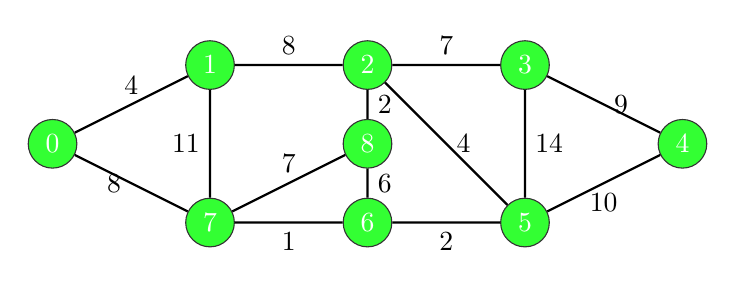
\begin{tikzpicture}
        % Define the nodes
        \node[circle, draw=black!80, fill=green!80, text=white, minimum size=15pt] (0) at (0,2) {0};
        \node[circle, draw=black!80, fill=green!80, text=white, minimum size=15pt] (1) at (2,3) {1};
        \node[circle, draw=black!80, fill=green!80, text=white, minimum size=15pt] (2) at (4,3) {2};
        \node[circle, draw=black!80, fill=green!80, text=white, minimum size=15pt] (3) at (6,3) {3};
        \node[circle, draw=black!80, fill=green!80, text=white, minimum size=15pt] (4) at (8,2) {4};
        \node[circle, draw=black!80, fill=green!80, text=white, minimum size=15pt] (5) at (6,1) {5};
        \node[circle, draw=black!80, fill=green!80, text=white, minimum size=15pt] (6) at (4,1) {6};
        \node[circle, draw=black!80, fill=green!80, text=white, minimum size=15pt] (7) at (2,1) {7};
        \node[circle, draw=black!80, fill=green!80, text=white, minimum size=15pt] (8) at (4,2) {8};

        % Draw the edges with weights
        \path[draw, thick] 
            (0) -- node[above] {4} (1)
            (0) -- node[left] {8} (7)
            (1) -- node[above] {8} (2)
            (1) -- node[left] {11} (7)
            (2) -- node[above] {7} (3)
            (2) -- node[right] {2} (8)
            (2) -- node[right] {4} (5)
            (3) -- node[right] {9} (4)
            (3) -- node[right] {14} (5)
            (4) -- node[below] {10} (5)
            (5) -- node[below] {2} (6)
            (6) -- node[below] {1} (7)
            (6) -- node[right] {6} (8)
            (7) -- node[above] {7} (8);
    \end{tikzpicture}
\end{center}
\end{frame}
\end{document}